\documentclass[10pt, reqno, letterpaper, twoside]{amsart}
\usepackage[margin=1in]{geometry}

\usepackage{amssymb, bm, mathtools}
\usepackage[usenames,dvipsnames,svgnames,table]{xcolor}
\usepackage[pdftex, xetex]{graphicx}
\usepackage{enumerate, setspace}
\usepackage{algorithm}
\usepackage{algpseudocode}
\usepackage{algorithm2e}
\renewcommand{\algorithmicrequire}{\textbf{Input:}}
\renewcommand{\algorithmicensure}{\textbf{Output:}}
\usepackage{float, colortbl, tabularx, longtable, multirow, subcaption, environ, wrapfig, textcomp, booktabs}
\usepackage{pgf, tikz, framed, url, hyperref}
\usepackage[normalem]{ulem}
\usetikzlibrary{arrows,positioning,automata,shadows,fit,shapes}
\usepackage[english]{babel}


\usepackage{biblatex} 
\addbibresource{refs.bib}

\usepackage{microtype}
\microtypecontext{spacing=nonfrench}

\usepackage{times}

\usepackage{xcolor}         % colors

\hypersetup{
    colorlinks,
    linkcolor={blue!50!black},
    citecolor={green!60!black},
    urlcolor={blue!80!black}
}


\title{cAlphaZero: A Reinforcement-Learning Sudoku Solver with Curriculum Scheduling}
\author{
Arunim Agarwal,
Zirun Han,
Alexander Kyimpopkin,
Lucas Klein
}

\begin{document}

\begin{abstract}
We propose \textit{cAlphaZero}, a reinforcement-learning and MCTS-based method inspired by AlphaZero to solve Sudoku as a step towards solving more general NP-complete problems with learning-based approaches.   We evaluate \textit{cAlphaZero} on $4 \times 4$ Sudoku to validate the performance of our method.  We find that the use of curriculum scheduling is key to achieving excellent model performance and stability during the training process. We also propose several additional modifications to the AlphaZero algorithm to adapt it for puzzle solving. \textit{cAlphaZero} can solve the $4 \times 4$ puzzles with a high degree of accuracy using only a few MCTS simulation steps. 
\end{abstract}

\maketitle

\section{Introduction}
When generalized to an $n \times n $ grid, Sudoku is an NP-complete problem \cite{yato2003complexity}.  This class of problems is most classically associated with problems such as Boolean satisfiability (SAT) and the Travelling salesman problem.  Prior work in Sudoku solvers has primarily relied on classical approaches, as well as a handful of modern learning-based approaches. \cite{mehta2021reinforcement}.  Prior literature has shown the ability to reformulate any NP-complete problem as a decision problem and thus a Boolean satisfiability problem.

Being an NP-complete problem, algorithms for solving $n\times n$ Sudoku are exponential with respect to $n$ and the run time quickly blows up with large Sudoku problems. Machine learning methods have been used in the past to approximately solve computationally intractable problems such as Go, molecule generation and data compression. \cite{Silver2018}\cite{bengio2021flow}\cite{yang2023introduction} In this paper, we show that neural networks can be effective at solving small Sudoku problems. We attempt to train two seperate models inspired by AlphaZero and GFlowNets respectively to solve Sudoku problems.

\subsection{Contributions}
We propose a neural network-accelerated Monte Carlo Tree Search (MCTS) method inspired by the AlphaZero algorithm to solve puzzles. We find that this algorithm can consistently solve $4 \times 4$ Sudoku games. We present several improvements to the canonical training regimen to adapt the algorithm for the single-player task of puzzle solving. We show that these modifications, including the use of entropy loss to optimize prediction confidence and scheduling the difficulty of training puzzles, enhance training stability and network performance.  We additionally experimented with Generative Flow Network (GFlowNet) based approaches \cite{bengio2023gflownet}\cite{jain2023biological}\cite{zhang2022generative}\cite{zhang2023unifying} but did not find them to be effective in solving puzzles. 

\section{Background}
 % NP-Complete problems represent a class of problems for which there is no current solution with polynomial run time, but whose solutions can be verified in polynomial time. Sudoku is commonly played with a 9x9 board which can be solved quickly however, in the general $n \times n$ case, Sudoku is NP-Complete and thus can be reduced to any other NP-Complete problem in polynomial time. 

\subsection{Monte Carlo Tree Search Algorithms}
Monte Carlo Tree Search (MCTS) is an algorithm used for decision processes and is used in game-theoretic applications to solve the game tree. MCTS works by expanding a search tree one node at a time, where each node represents a state in the game and each branch represents an action by which the game transitions to a new state.

AlphaZero\cite{Silver2018}\cite{10.1038/nature16961}, an game-playing approach built on MCTS and trains solely through self-play without human knowledge, maintains
\begin{itemize}
    \item $Q(s,a)$: the expected reward of a state-action pair $(s,a)$
    \item $N(s,a)$: the number of times action $a$ has been searched from state $s$
    \item $P(s,a)$: the initial probability of taking action $a$ from state $s$ returned from the model's policy
\end{itemize}
$Q(s,a)$ and $P(s,a)$ are estimated by a neural network with a value head and policy head respectively. AlphaZero uses a variant of the PUCT algorithm\cite{puct} to determine the upper confidence bound (UCB) $U$
\begin{align}
   U(s,a) &= Q(s,a) + c_{puct}P(s,a) \cdot \frac{\sqrt{\sum_bN(s,b)}}{1+N(s,a)} \\
   a_t &= \mathop{\mathrm{argmax}}_a \  U(s,a)
\end{align}
and thus select actions from each node, where $c_{puct}$ is a hyperparameter that is used to balance exploration and exploitation. 

Our approach slightly modifies this UCB score by introducing a small additive constant (in practice, $0.5$) to the UCB score for any action that has not yet been explored. We have found that this is a simple but effective way to prevent an overconfident policy network from inducing poor MCTS searches and overfitting to these poor searches in the early stages of the curriculum-scheduled training process (e.g. 2-blank puzzles) when the value net is relatively unimportant.

\subsection{GFlowNets}
Flow networks consist of a directed graph with sources, sinks, intermediate nodes and edges carrying some amount of flow between them. Flow networks can be thought of like network of pipes with water flowing through them. Each sink, $x$ represents a terminal state has an "out-flow", $R(x)$ which represents the reward of that terminal state. For our purposes there will be a singular source $s_0$ which is the initial state. We will denote $F(s,a)=f(s,s')$ as the flow between states $s$ and $s'$ where $T(s,a)=s'$ is the state reached by taking action $a$ from state $s$. Using this formulation of actions and states one can obtain a Markov Decision Process (MDP) with the policy
\begin{align}
    P(s,a) = \frac{F(s,a)}{\sum_{a'} F(s,a')}
\end{align}

where following policy $P$ from $s_0$ leads to terminal state $x$ with probability $R(x)$. \cite{bengio2023gflownet} %We can define a \textit{valid} flow for a state $s'$ as one where the in-flow is equal to the out-flow. We will denote the flow of state $s'$ as $F(s')$. A \textit{valid} flow must satisfy

%\begin{align}
%    F(s') &= {\sum_{s,a s.t T(s,a)=s'}}F(s,a) \\
%    F(s') &= R(s') + \sum_{a'\in \mathcal{A}(s')}F(s',a')
%\end{align}
%where $\mathcal{A}(s')$ is the set of actions for state $s'$. In most problems explicitly maintaining the entire flow network is intractable, however we can approximate this network by optimizing an objective which minimizes square difference between the in-flow and out-flow. 
%\begin{align}
%    L_{\theta, \epsilon}(\tau) = \sum_{s' \in \tau \setminus \{s_0\}} \left( 
%    \log \left[ \frac{\epsilon + s,a : T(s,a) = s'}{\sum \exp \left( \log F_{\theta}(s,a) \right)} \right] - 
%    \log \left[ \frac{\epsilon + R(s') + \sum_{a' \in A(s')} \exp \left( \log F_{\theta}(s',a') \right)}{\sum \exp \left( \log F_{\theta}(s',a') \right)} \right] 
%\right)^2
%\end{align}
Compared to other methods GFlowNets generate more diverse trajectories because they generate trajectories with probability proportional to reward compared to methods which try to maximize reward.

\section{Related Work}

Sudoku is a game with a rich history \cite{sudokuHistoryWayback} and myriad algorithmic approaches as well as many formulations. \cite{10.1587/transfun.e100.a.2641}

\subsection{Sudoku Solvers}
Numerous Sudoku solvers based on backtracking \cite{chi2013techniques}\cite{10.29007/79mc} exist, with recent \cite{10.1109/iadcc.2014.6779291} \cite{10.5220/0001659502460254}\cite{10.1007/s11786-017-0322-4} literature showing ongoing work in this area towards establishing a baseline.  Recent approaches in Sudoku have concentrated on classical approaches using a mixture of different approaches, ranging from graph theory\cite{10.46460/ijiea.982908} to alternating projections\cite{10.5120/ijca2019918439} and extensions to higher dimensions \cite{10.1007/s11786-017-0322-4}.  These approaches have shown significant promise in rapidly solving classical $9\times 9$ Sudoku problems.

\subsection{Reinforcement Learning}

Prior literature in reinforcement learning has shown the efficacy of curriculum scheduling \cite{10.24963/ijcai.2017/757}, suggesting its efficacy in solving challenging problems.  More recent advancements in the field \cite{Silver2018} have highlighted the efficacy of MCTS-based approaches, achieving superhuman performances in combinatorially challenging games such as Chess, Go, and Shogi.  These advancements have been further expanded \cite{Schrittwieser_2020} to generalize to games with unknown rule structures. Work in MCTS-based puzzle solvers has made strides, using computational approaches  \cite{Kiarostami2021}, and showing substantial efficacy in solving a broad class of puzzles using probabilistic searches. 

\section{Approach}
\subsection{Motivation for NN-Accelerated MCTS}

Two computationally expensive aspects of a traditional MCTS algorithm are that the game must be ``rolled out" to an end state for a reward to be assigned and that a large number of nodes must be explored to ensure that the empirical selection policy is accurate. In our algorithm, at each game state $s$, we instead use a neural network to predict a policy $\pi_s$  and an evaluation $v_s$. As such, when we conduct an MCTS search at $s$, $\pi_s$ is used as the prior distribution to ``hot start" the search process by focusing the search on the most promising actions. Additionally, instead of rolling out to an end state, we can assign $v_{s'}$, the expected reward, when we encounter an unexplored node $s'$ in the game tree. Theoretically and empirically, this guided search process reduces the computation required to solve the puzzle. 

\subsection{Learning Process}

The learning process we used can be broken down into two main components: game generation and network training. During game generation, a large number of games are played using the neural-MCTS algorithm. Each game generates a chain of data in the form of $(s, p_s, r)$ where $s$ is a board position, $p_s$ is the empirical policy after conducting a number of MCTS simulations, and $r$ is the reward at the end state of the chain of actions selected by the algorithm. For our algorithm, we chose to use a constraint satisfaction reward with the form
\begin{equation}
    r(s^\mathrm{T}) = \frac{1}{N} \sum_{i=0}^N c_i(s^\mathrm{T})
\end{equation}
where $c_i \in \{0,1\}$ is an indicator function for the $i$th constraint for a solved game. The game is completely solved when the reward for the terminal state, $r(s^\mathrm{T})=1$. For $n \times n$ Sudoku, there are $3n$ total constraints for the rows, columns, and subgrids. 

After each game is played, we exploit the symmetries inherent to Sudoku to augment the data, including rotations of the board, permutations between rows within their row-group, permutations of entire row-groups. We also partially exploit the symmetry of permuting the numbers associated with each square, but as the board size $n$ increases, using all such permutations becomes increasingly intractable by the combinatorial explosion of such transformations. The empirical policies are also transformed correspondingly, while the rewards are held constant, to generate our augmented $(s, p_s, r)$ tuples. Through this process, we're able to massively increase the data available to train our policy and value network, without needing to play an intractable number of games. 

The generated and augmented data is then fed into the neural network which is trained on the loss function
\begin{equation}
    \ell (p_s, \pi_s, r, v_s) = \lambda (r - v_s)^2 - p_s^\top \log(\pi_s) + \xi \pi_s^\top \log \pi_s
\end{equation}
where $\pi_s$ and $v_s$ are the network-predicted policy and value respectively. Comparing this to the AlphaZero loss:
\begin{equation}
    \ell_{AZ} (p_s, \pi_s, r, v_s) = (r - v_s)^2 - p_s^\top \log(\pi_s)
\end{equation}

\begin{wrapfigure}{r}{0.3\textwidth} % This will wrap the text around the figure to the right
    \centering
    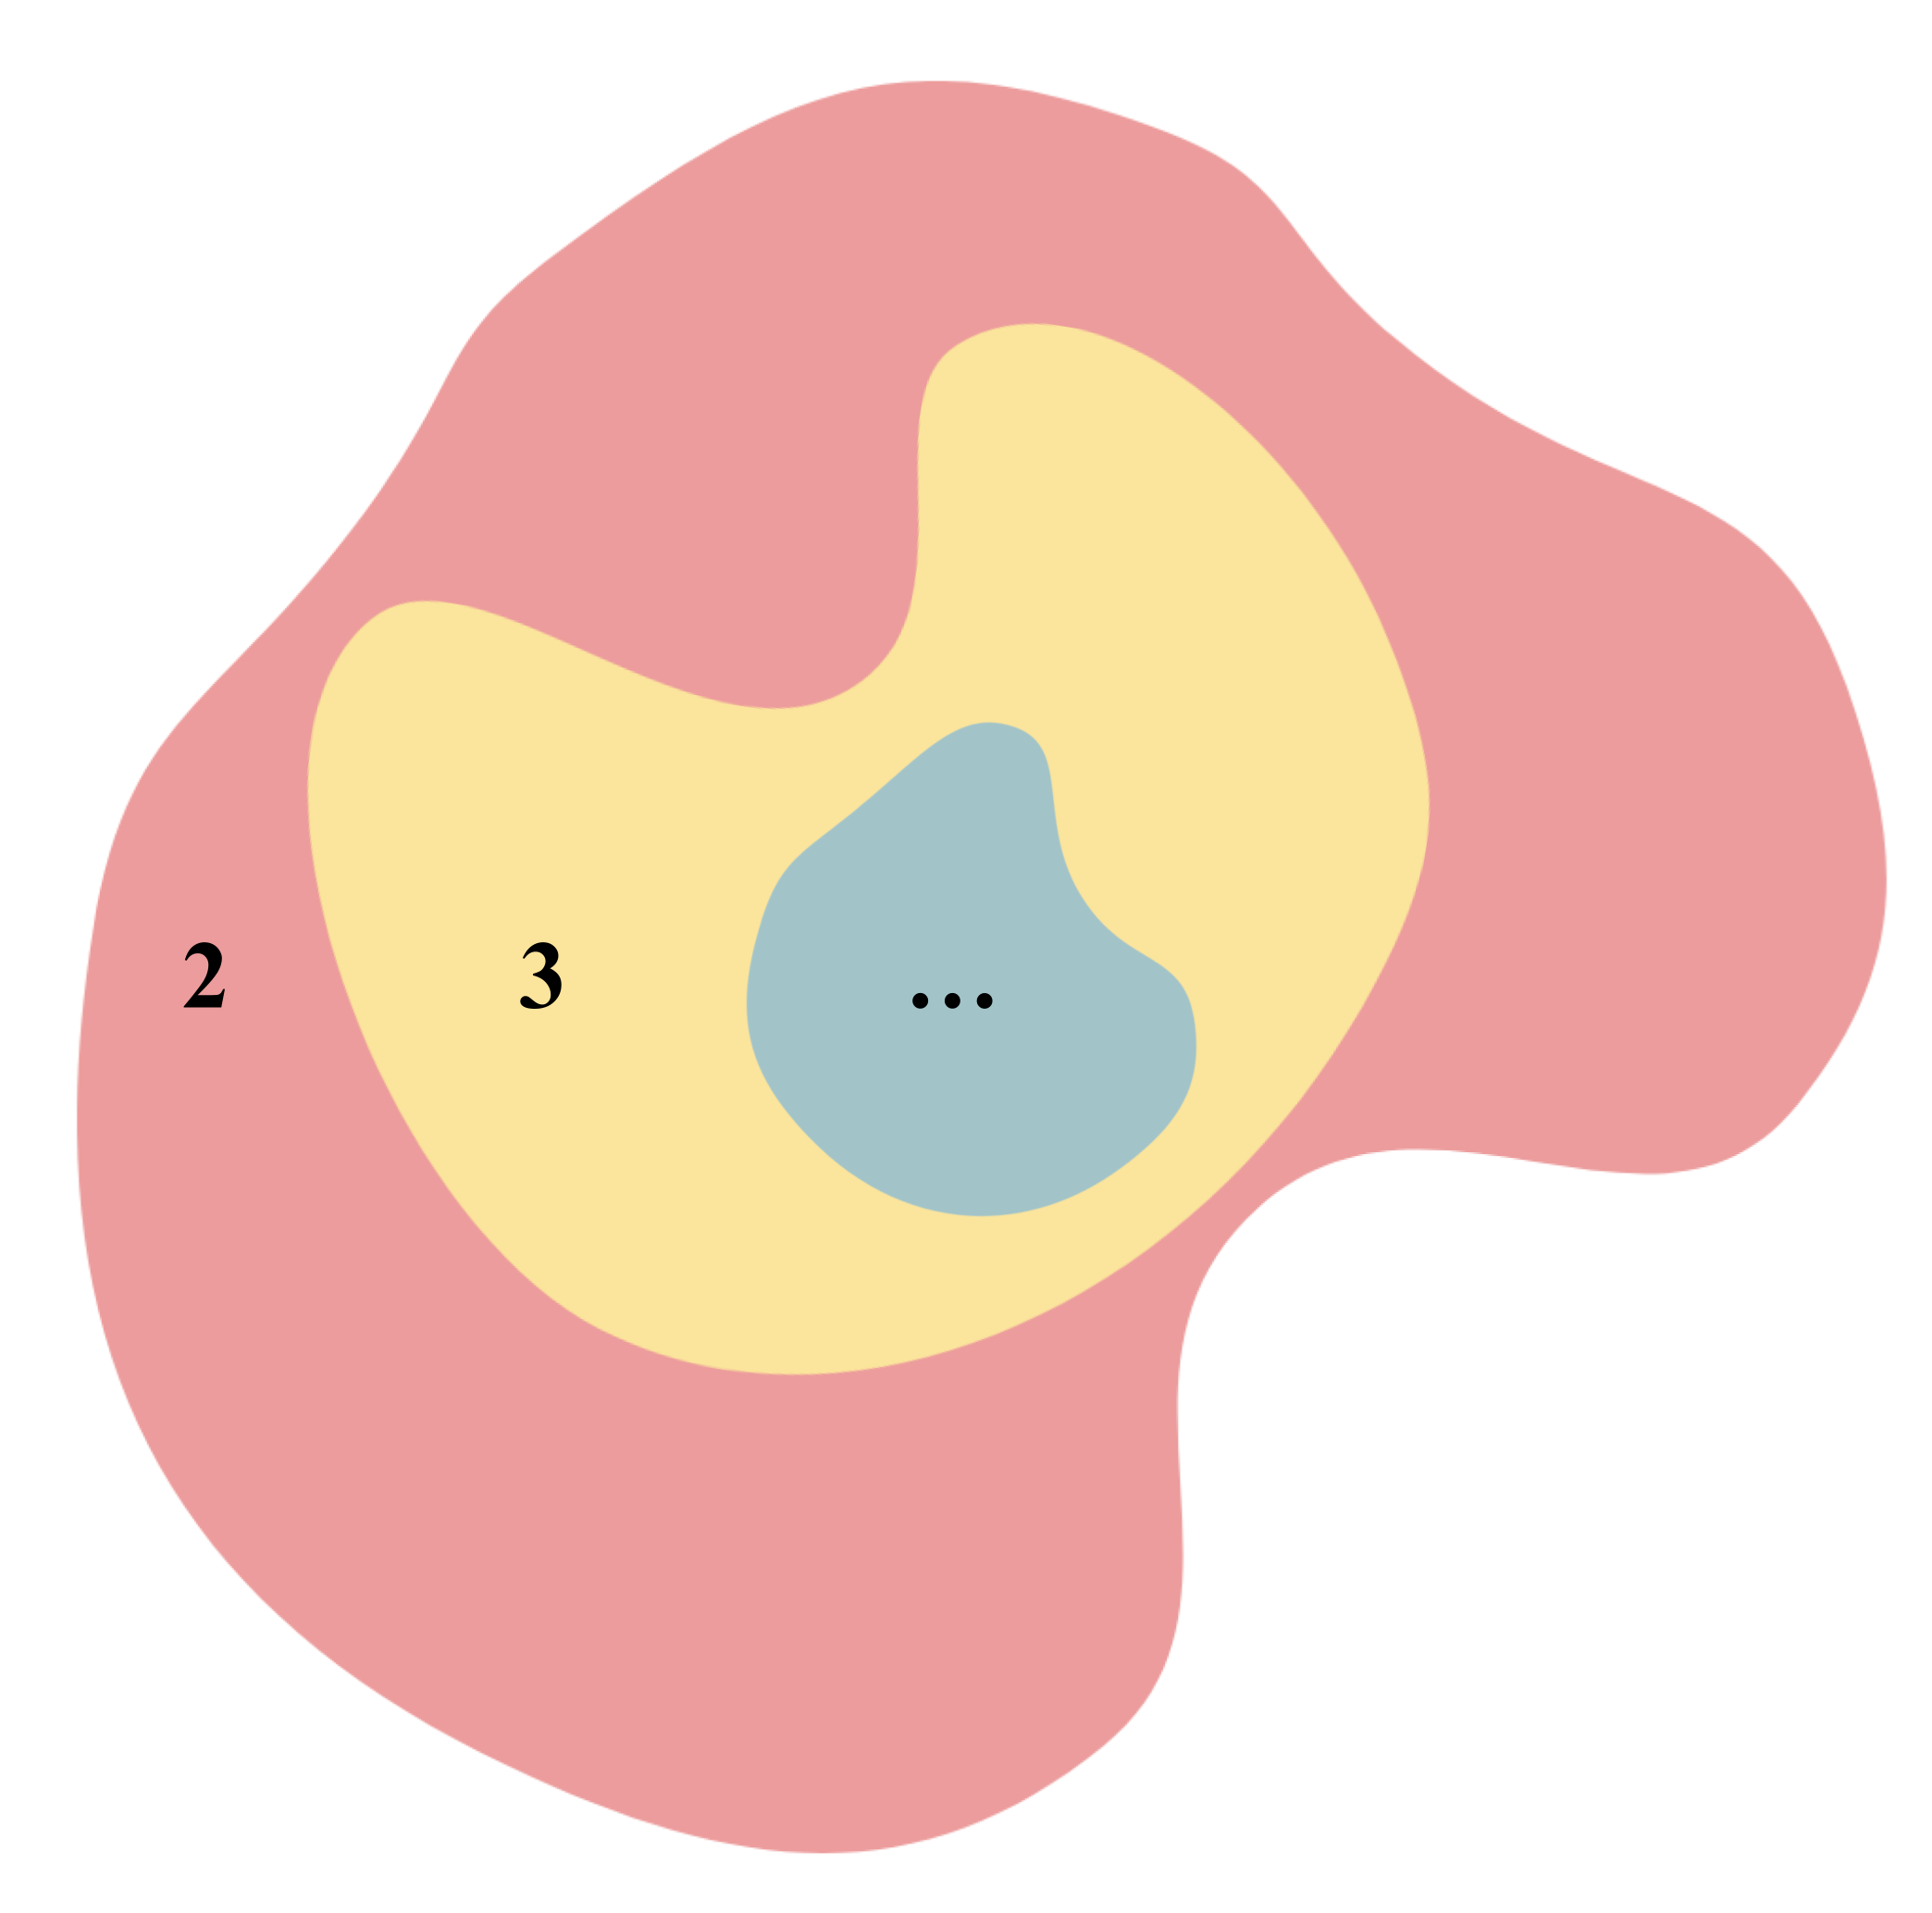
\includegraphics[width=0.3\textwidth]{images/blobs.png}
    \caption{Regions of model space which are able to solve puzzles of increasing difficulty, in our case, increasing numbers of blanks.}
    \label{fig:blobs}
\end{wrapfigure}

we have added a scaling factor $\lambda = 100 $ to balance the magnitude of the value and policy loss. Additionally, we have added a third term that is equal to the entropy of the network policy scaled by a factor $\xi$. The motivation for adding this term is two-fold. First, this stabilizes the training process at the beginning of our runs, as we will discuss in the next section. Further, this can be used to control the network's confidence at different stages of the game. A high policy entropy corresponds to low confidence and more diverse searching, which is optimal for the early game where there are many correct moves. On the other hand, the network should be confident near the endgame for efficiency. 

\subsection{Curriculum Scheduling}

A major component of our training process is the scheduling of puzzle difficulties. Training directly on full-difficulty Sudoku puzzles resulted in the network failing to learn a meaningful policy.

Drawing on existing work in curriculum learning and reinforcement learning curriculum schedules, we introduced a curriculum schedule detailed in \hyperref[algo:algo1]{Training Algorithm}. Specifically in the case of Sudoku, intuitively, models $\{\mathcal{M}_{n+1}\}$ which can solve $n+1$-blank Sudoku puzzles are a subset of models $\{\mathcal{M}_{n}\}$ able to solve $n$-blank Sudoku puzzles. This is visualized in \ref{fig:blobs}.


Our curriculum gradually ramps the difficulty, beginning with two-blank puzzles and increasing the number of blank squares by one once the model has attained a specific accuracy or trained for a maximum number of iterations.

MCTS lends itself well to this curriculum schedule, since the process of MCTS naturally provides a gradual transition when we increase the number of blanks. We can see this by considering the $n$-blank game to be a child node of many $(n+1)$-blank games which are one square removed, and noting that when MCTS reaches the next layer, there are only $n$ blanks. As such, the covariate shift the network experiences is gradual, improving the stability of the training process.  We suggest that this behavior is caused by the size of the Rashomon Set\cite{Semenova_2022} shrinking substantially for each increase in the number of blanks. 

\section{Experimental Results}

In the section below, we plot and detail the results of our training process using \textit{cAlphaZero} on $4 \times 4$ Sudoku games on multiple architectures, and we present a negative result of poor training convergence without the use of curriculum scheduling. 

We can now see the effect of our previously mentioned change in the size of the Rashomon set associated with our problem over the course of the curriculum. This set, defined to be the set of almost-equally-accurate models, is largest for the simplest problem of filling in two blanks and much smaller for each subsequent model. Beginning the training process with two-blank games therefore presents a large target that is easy to find. We see this in the sharp drop in loss and corresponding increase in accuracy in the first steps of Figure \ref{fig:MLP-score-cAlphaZero}. Then, as blanks are added in, we see the losses hold steady on the order of $0.1$ and $0.001$, while the accuracy stays clear of $95\%$. The training run without any curriculum scheduling, on the other hand, provides a stark contrast and a strong indication of a negative result. This test was run on a modest difficulty of $8$ blanks, and as seen in Figure \ref{fig:MLP-loss-no-curriculum} and \ref{fig:MLP-score-no-curriculum}, the loss initially drops, but hovers about an order of magnitude above the losses with curriculum scheduling. Even the initial drop in loss is deceiving, as the limiting policy loss of 4.1 roughly corresponds to predicting $P(s,a)=\frac{1}{\text{\# actions}}$, i.e. random policy. Following the analogy of decreasing size of solvers in model space, a training process without curriculum scheduling is unable to locate the small space of models able to make progress on $8$-blank puzzles, let alone solve them fully. Iteratively guiding the process towards the correct area in model space, however, empirically is shown to work. 

The validation losses plotted in Figures \ref{fig:MLP-loss-cAlphaZero}, \ref{fig:MLP-loss-no-curriculum} are evaluated for the neural network with respect to a holdout set of generated game data after each epoch. We do not provide overall results on ``test" data, as the augmentation process can transform boards in the training dataset to boards in the validation set, making the construction of a holdout set a bit more intensive. Despite these constraints, we argue that our model is generalizing by observing a few key points. First, the validation metrics on the holdout data after each epoch closely track the training loss, indicating that during each epoch, we are not overfitting to the provided data. Second, we can observe the drop in accuracy at each increase in number of blanks. By decreasing the number of blanks, we induce a shift in the overall distribution, and we find that the percentage of perfect games stays above $90\%$, indicating generalization.
% Critical thinking says the paragraph above is not rigorous. MCTS could very well search the 10 * 4 = 40 options, get back into a distribution it is overfit to, perform well on that, and then do well on the "new distribution" as a result. Not having a test set is obviously not rigorous, and in hindsight, we very easily could have chosen a few random boards, applied the transformations, and removed those transformed boards from the dataset as well, since transformations are symmetric... Ran out of time implement the test set but leaving this comment in for the sake of transparency.

We provide two experimental training runs with self-attention-based architectures with learnable position encoding. This is motivated by the ability of self-attention layers to capture long-range dependencies while using significant weight sharing compared to MLPs. Empirically, we find that the smaller of these models ($80\%$ smaller than the MLP) achieves similar losses but struggles towards the end of training, while the larger model ($22\%$ smaller) has no trouble maintaining low loss throughout training. See corresponding loss and score curves in Figure \ref{fig:attention-loss} in the Appendix.
% Possible that the observed differential could be made up by giving the smaller (thus lower capacity) model a more appropriate amount of data / training time--I feel like we learned about this but didn't implement it. Again, leaving this in for transparency / so others can improve. 

\begin{figure}[ht]
    \centering
    % Subfigure 1
    \begin{subfigure}[b]{0.45\textwidth}
        \centering
        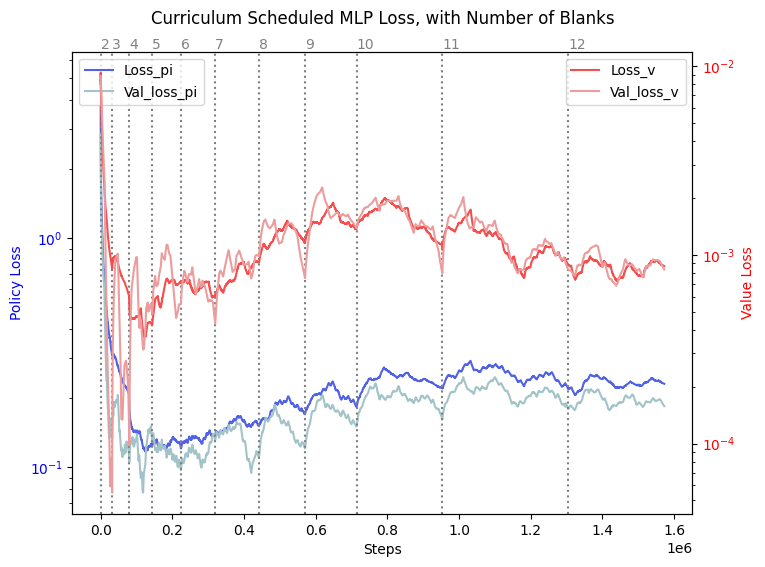
\includegraphics[width=0.9\textwidth]{images/Curriculum Scheduled MLP Loss.png}
        \caption{Policy and value training loss curves for an MLP architecture using \textit{cAlphaZero}}
        \label{fig:MLP-loss-cAlphaZero}
    \end{subfigure}
    \hfill
    % Subfigure 2
    \begin{subfigure}[b]{0.45\textwidth}
        \centering
        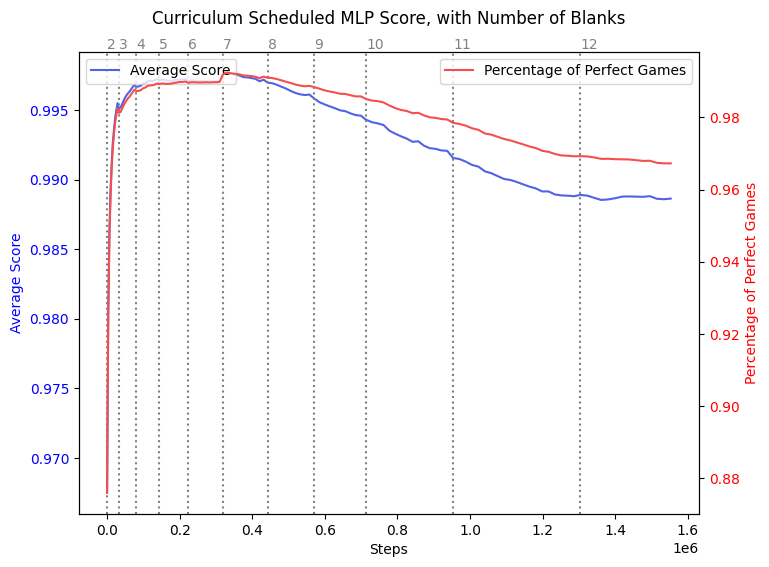
\includegraphics[width=0.9\textwidth]{images/Curriculum Scheduled MLP Score.png}
        \caption{Associated score metrics during the \textit{cAlphaZero} training run}
        \label{fig:MLP-score-cAlphaZero}
    \end{subfigure}
    
    % Subfigure 3
    \begin{subfigure}[b]{0.45\textwidth}
        \centering
        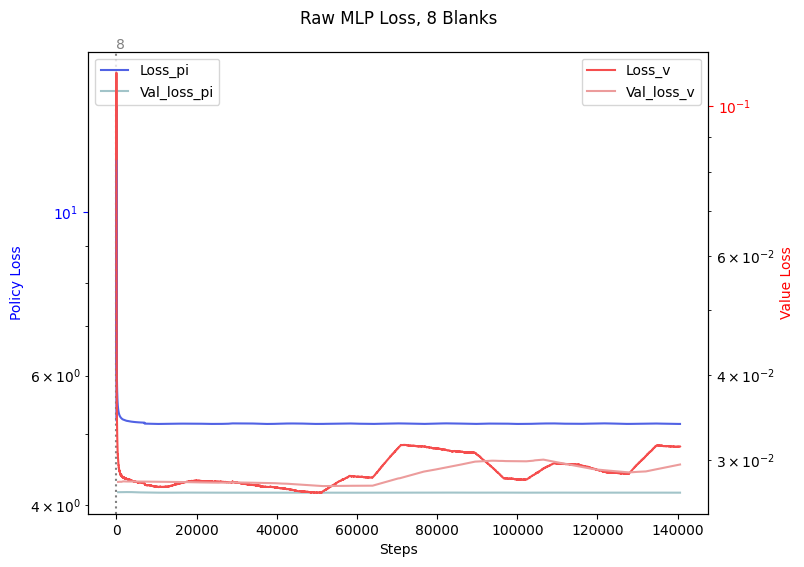
\includegraphics[width=0.9\textwidth]{images/Raw MLP Loss.png}
        \caption{Policy and value training loss curves without curriculum scheduling}
        \label{fig:MLP-loss-no-curriculum}
    \end{subfigure}
    \hfill
    % Subfigure 4
    \begin{subfigure}[b]{0.45\textwidth}
        \centering
        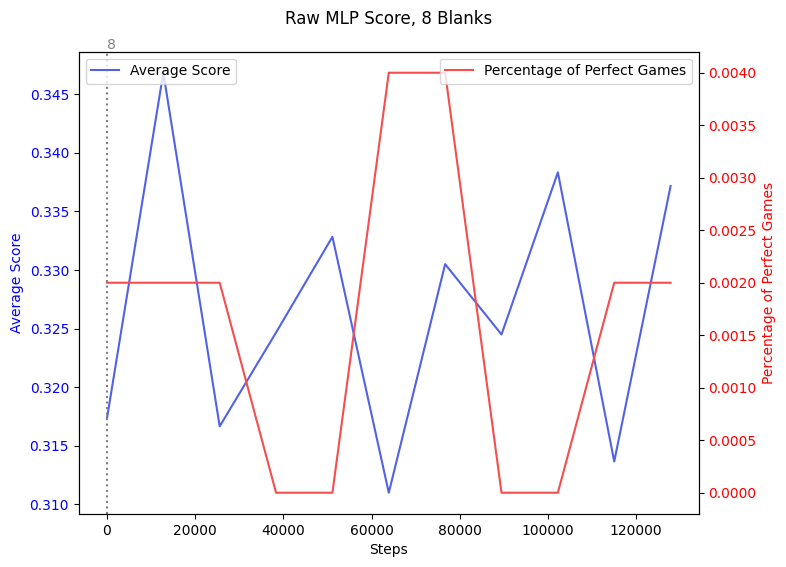
\includegraphics[width=0.9\textwidth]{images/Raw MLP Score.png}
        \caption{Associated score metrics during the same training run without curriculum scheduling}
        \label{fig:MLP-score-no-curriculum}
    \end{subfigure}

    \caption{Comparative analysis of MLP architecture in \textit{cAlphaZero} training with and without curriculum scheduling.}
    \label{fig:MLP-loss}
\end{figure}

\begin{figure}
    \centering
    \begin{subfigure}{0.45\textwidth}
        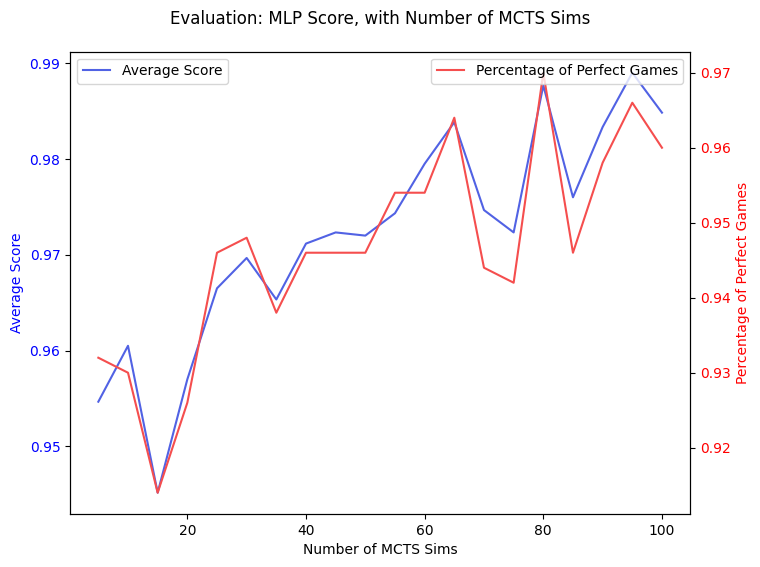
\includegraphics[width=0.8\linewidth]{images/eval_mlp.png}
        \caption{Evaluation of the MLP architecture using \textit{cAlphaZero} after the training shown in Figure \ref{fig:MLP-loss-cAlphaZero}}
    \end{subfigure}
    \hfill
    \begin{subfigure}{0.45\textwidth}
        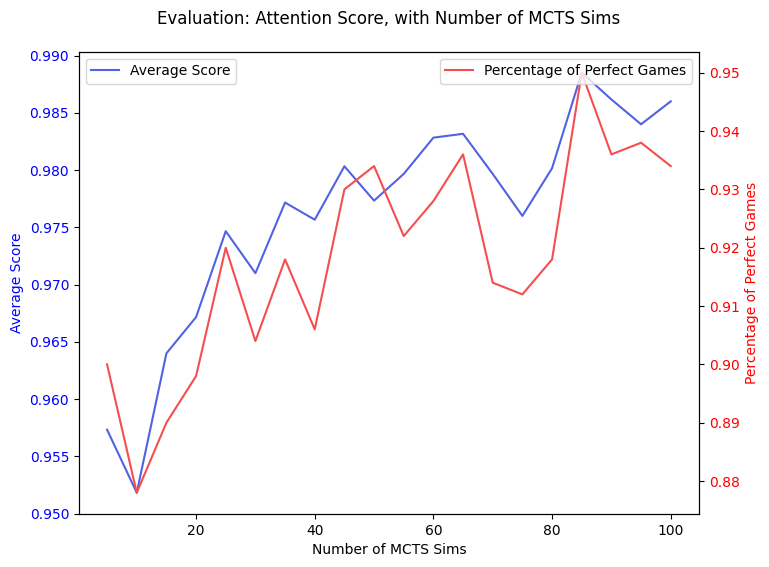
\includegraphics[width=0.8\linewidth]{images/eval_attention.png}
        \caption{Evaluation of the attention architecture with hidden layer size 512 using \textit{cAlphaZero} corresponding to Figure \ref{fig:attention-512-loss}}
    \end{subfigure}
    \caption{Post-training evaluation of MLP and attention-based architectures using \textit{cAlphaZero}}
    \label{fig:MLP-loss}
\end{figure}


We find that GFlowNet-based methods do not learn to solve Sudoku puzzles within a reasonable time.   We experimented with both detailed balance and trajectory balance losses in order to address this challenge. \cite{https://doi.org/10.15488/13422}.  The model learned some aspects of the 9x9 puzzles, reducing the trajectory balance loss from $55.76$ to $19.029$ after $5000$ episodes, but failed to materially improve on those results.  Given our observed successes with curriculum scheduling in \textit{cAlphaZero}, a curriculum scheduled GFlowNet may be able to substanially improve on these results.

\section{Discussion}

We find that our AlphaZero \cite{Silver2018} based approach to learning solutions to Sudoku problems is able to consistently solve small problems when presented with a scheduled curriculum, drawing on prior literature in curriculum scheduling \cite{https://doi.org/10.15488/13422}.  We additionally attempted to solve Sudoku puzzles with gflownets \cite{bengio2023gflownet}, but consistently encountered challenges around sample efficiency as well as small models inability to converge to a meaningfully low error.  

Although we only experimented with single-try runs (i.e. no explicit backtracking), the algorithm can be easily adapted to deterministically obtain the answer using many runs. To do this, we perform a single run, and if the end state does not solve the puzzle, we set the associated UCB score to zero and return to the root node of the search tree.

\section{Future work}

For this work, we focused on smaller $4\times 4$ puzzles in our reinforcement learning-based approach due to computational challenges in our reinforcement-learning-based regime. Nevertheless, the ability to generalize this algorithm to a broader context hinges on its ability to generalize to larger puzzles. We aim to extend this work to perform game generation in parallel and therefore hope to more closely focus on self-attention-based models. This is because fully connected MLPs will become computationally challenging to train as the state and action spaces scale rapidly with puzzle size. Here, we hope to test novel sub-quadratic attention approaches based on alternative paradigms such as Monarch Matrices \cite{fu2023monarch} to evaluate their relative efficacy for this probabilistic puzzle-solving paradigm. While GFlowNets were not meaningfully able to solve $9\times 9$ Sudoku problems, switching them to a curriculum-scheduled version following our promising results with \textit{cAlphaZero} presents a direction for further exploration. We are excited about the performance of probabilistic solvers for Sudoku, and hope to extend our approach to Boolean Satisfiability (SAT) and the Traveling Salesman Problem. 

\clearpage
\printbibliography

\newpage
\appendix
\section{Attention-based Architecture Results}

\begin{figure}[ht]
    \centering
    % Subfigure 1
    \begin{subfigure}[b]{0.45\textwidth}
        \centering
        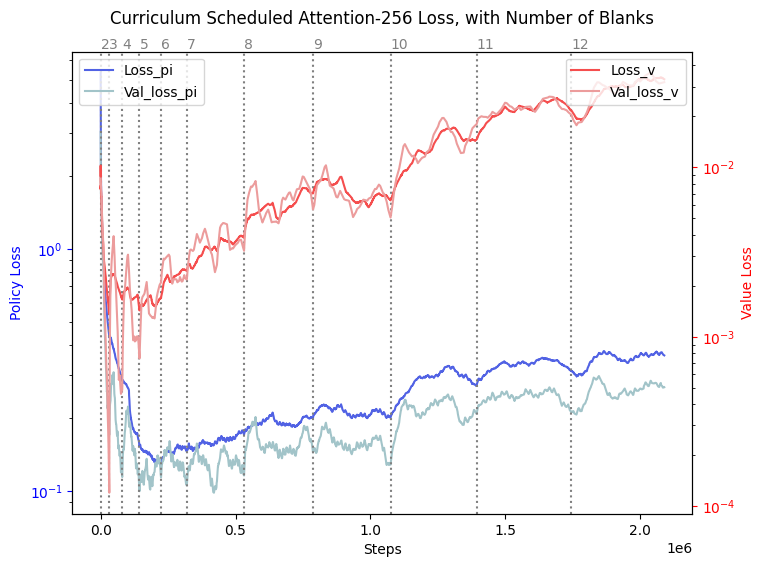
\includegraphics[width=0.9\textwidth]{images/Curriculum Scheduled Attention-256 Loss.png}
        \caption{Policy and value training loss curves for attention architecture with hidden layers of size 256 using \textit{cAlphaZero}}
        \label{fig:attention-256-loss}
    \end{subfigure}
    \hfill
    % Subfigure 2
    \begin{subfigure}[b]{0.45\textwidth}
        \centering
        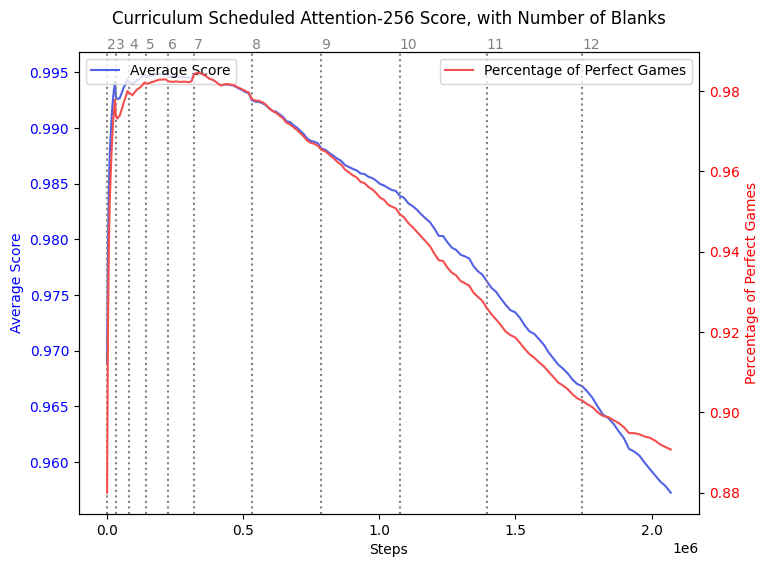
\includegraphics[width=0.9\textwidth]{images/Curriculum Scheduled Attention-256 Score.png}
        \caption{Associated score metrics during the cAlphaZero training run with hidden layers of size 256}
        \label{fig:attention-256-score}
    \end{subfigure}
    
    % Subfigure 3
    \begin{subfigure}[b]{0.45\textwidth}
        \centering
        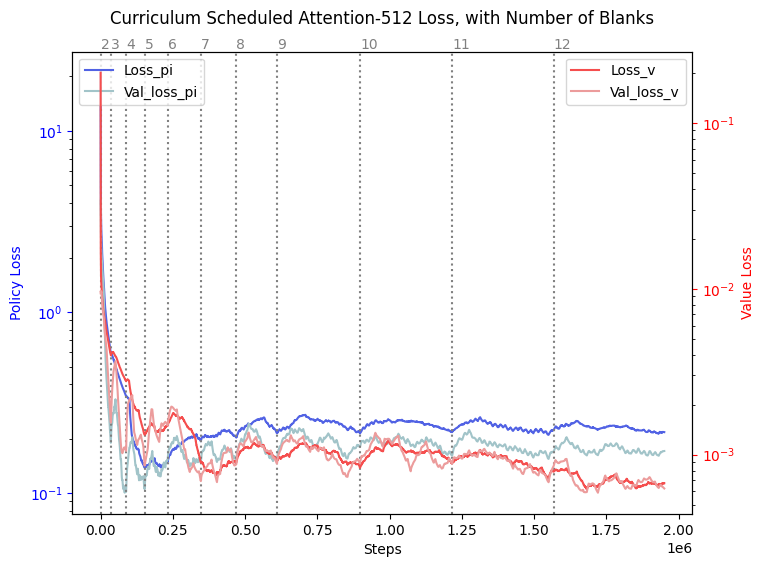
\includegraphics[width=0.9\textwidth]{images/Curriculum Scheduled Attention-512 Loss.png}
        \caption{Policy and value training loss curves for attention architecture with hidden layers of size 512 using cAlphaZero}
        \label{fig:attention-512-loss}
    \end{subfigure}
    \hfill
    % Subfigure 4
    \begin{subfigure}[b]{0.45\textwidth}
        \centering
        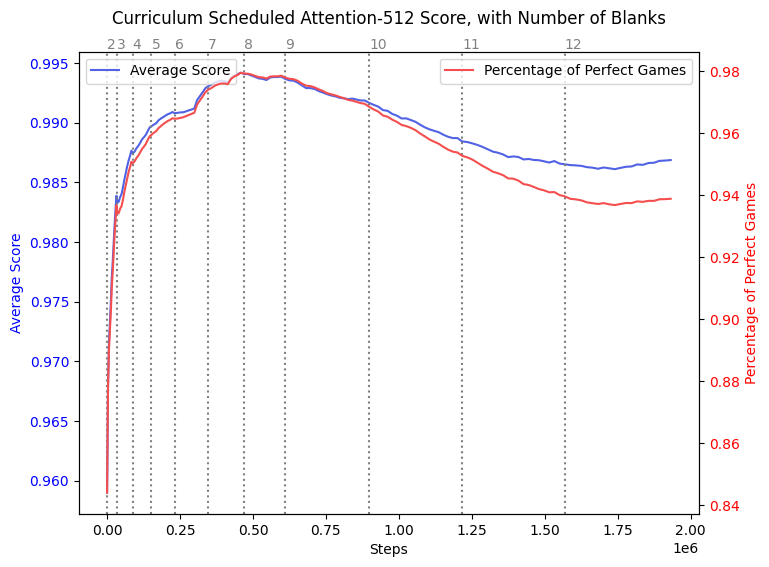
\includegraphics[width=0.9\textwidth]{images/Curriculum Scheduled Attention-512 Score.png}
        \caption{Associated score metrics during the cAlphaZero training run with hidden layers of size 512}
        \label{fig:attention-512-score}
    \end{subfigure}

    \caption{Comparative analysis of attention-based architecture in cAlphaZero training with hidden layers of size 256 and 512.}
    % An earlier (submitted-to-the class) version had plots that were not representative of proper training runs. These should be correct.
    \label{fig:attention-loss}
\end{figure}
\newpage
\section{Algorithmic Approach to Training}

\begin{figure}[h]
\begin{algorithm}[H]
\caption{\hspace{-1mm}\textbf{:} \textbf{\textit{cAlphaZero} Training Algorithm with Curriculum Scheduling}}

\SetKwInOut{Input}{Inputs}
\SetKwInOut{Begin}{Begin}
\SetKwInOut{Output}{output}

\label{alg:cap}
\begin{algorithmic}[1]
\hspace{-13mm}

\Input{
\newline %\newline
Neural Network $\theta$ \newline

$\mathcal{X}$ \gets {Set \hspace{1mm} of \hspace{1mm} puzzles} \newline

u \gets {Upper \hspace{1mm} bound \hspace{1mm} of \hspace{1mm} number \hspace{1mm} of \hspace{1mm} squares \hspace{1mm} to \hspace{1mm} solve \hspace{1mm} for \hspace{1mm} curriculum \hspace{1mm} schedule } \newline

$\mathcal{f(n, \theta)}$ \gets{Function \hspace{1mm } to \hspace{1mm } generate \hspace{1mm } data/trajectories \hspace{1mm } given \hspace{1mm } model }
\newline


\gamma \gets{Quality \hspace{1mm} metric \hspace{1mm } to\hspace{1mm } increase \hspace{1mm } number \hspace{1mm } of \hspace{1mm } squares \hspace{1mm } to \hspace{1mm } solve}

}

\newline
\newline

%\hspace{-13mm}\textbf{Output:} 

%\Begin{\newline
\textbf{while} \hspace{1mm} number \hspace{1mm} of \hspace{1mm} blanks \hspace{1mm } n \le u$: \newline\newline
%\NoDo
%\algorithmicforeach \hspace{1mm} {task \hspace{1mm} $t \in \mathcal{T}$\newline
    \indent\textbf{for} x_i \in \mathcal{X} \newline
     \indent\indent $d_i = f(n \hspace{1mm}  \vert \hspace{1mm} \theta, x_i)$ 
     \algorithmiccomment{Generated trajctories of board state, empirical policy and reward}\newline
     
        \indent\textbf{end for} \newline\newline
        $\indent \alpha = \text{TrainNet}(\theta, d)$ \algorithmiccomment{Accuracy of training policy network on empirical value of moves}\newline\newline
        
        \indent \textbf{if} \alpha > \gamma: \algorithmiccomment{Curriculum scheduling} \newline$
        \indent\indent $n' \gets{n+1}$ 
   
 %}
\end{algorithmic}
\end{algorithm}
\caption{The \textit{cAlphaZero} training algorithm with curriculum scheduling and the assumed notation.}
\label{algo:algo1}
\end{figure}

\end{document}